\documentclass[conference]{IEEEtran}
\usepackage{graphicx}
\usepackage{amsmath}
\usepackage{algorithm}
\usepackage{algpseudocode}
\usepackage{tikz}
\usepackage{booktabs}
\usepackage{multirow}
\usepackage{pgfplots}
\usepackage{pgf-pie}
\usepackage{url}

\usetikzlibrary{positioning,shapes,arrows.meta,calc}

\begin{document}

\title{Migración de Arquitecturas Monolíticas a Microservicios: \\ Análisis Comprehensivo y Estrategias Avanzadas}

\author{
\IEEEauthorblockN{Juan Carlos Rodríguez-Martínez}
\IEEEauthorblockA{\textit{Departamento de Ingeniería de Software} \\
\textit{Universidad Tecnológica de Innovación Digital} \\
Ciudad de México, México \\
jc.rodriguez@utid.edu.mx}
}

\maketitle

\begin{abstract}
La transformación digital exige arquitecturas de software más ágiles y escalables. Este artículo presenta un análisis profundo de la migración desde arquitecturas monolíticas tradicionales hacia microservicios, explorando metodologías, desafíos técnicos y estrategias de implementación. Mediante un estudio comparativo de casos empresariales de alto impacto, se demuestran los beneficios cuantitativos y cualitativos de esta transición arquitectónica. Además, se incluye un análisis detallado de herramientas clave y una proyección de tendencias futuras en arquitectura de software.
\end{abstract}

\begin{IEEEkeywords}
Microservicios, Arquitectura de Software, Transformación Digital, DevOps, Escalabilidad, Contenerización, Kubernetes, Resiliencia.
\end{IEEEkeywords}

\section{Introducción}

\subsection{Panorama Actual de las Arquitecturas de Software}
La evolución tecnológica ha transformado radicalmente los paradigmas de desarrollo de software. Las arquitecturas monolíticas, predominantes durante décadas, enfrentan limitaciones críticas en entornos de alta demanda y rápida innovación. 

\vspace{1em}

\begin{figure}[htbp]
\centering
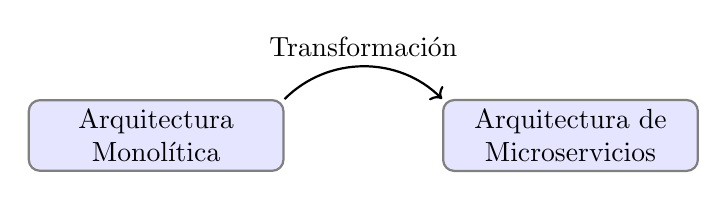
\begin{tikzpicture}
\tikzset{
    block/.style={rectangle, draw=black!50, thick, fill=blue!10, text width=3cm, text centered, rounded corners, minimum height=2em}
}
\node[block] (monolith) at (0,0) {Arquitectura Monolítica};
\node[block, right=2cm of monolith] (microservices) {Arquitectura de Microservicios};

\draw[thick,->] (monolith.north east) to[bend left=45] node[midway,above] {Transformación} (microservices.north west);
\end{tikzpicture}
\caption{Transición Arquitectónica: De Monolitos a Microservicios}
\label{fig:architectural_transition}
\end{figure}

\subsection{Motivaciones para la Migración}
Las principales razones que impulsan la migración incluyen:

\begin{itemize}
    \item \textbf{Escalabilidad:} Necesidad de manejar cargas dinámicas.
    \item \textbf{Resiliencia:} Mejor tolerancia a fallos.
    \item \textbf{Flexibilidad:} Capacidad de adoptar múltiples tecnologías.
    \item \textbf{Agilidad en DevOps:} Mejoras en los tiempos de despliegue.
    \item \textbf{Reducción de Costos Operativos:} Aprovechamiento de recursos.
\end{itemize}

\begin{figure}[htbp]
\centering
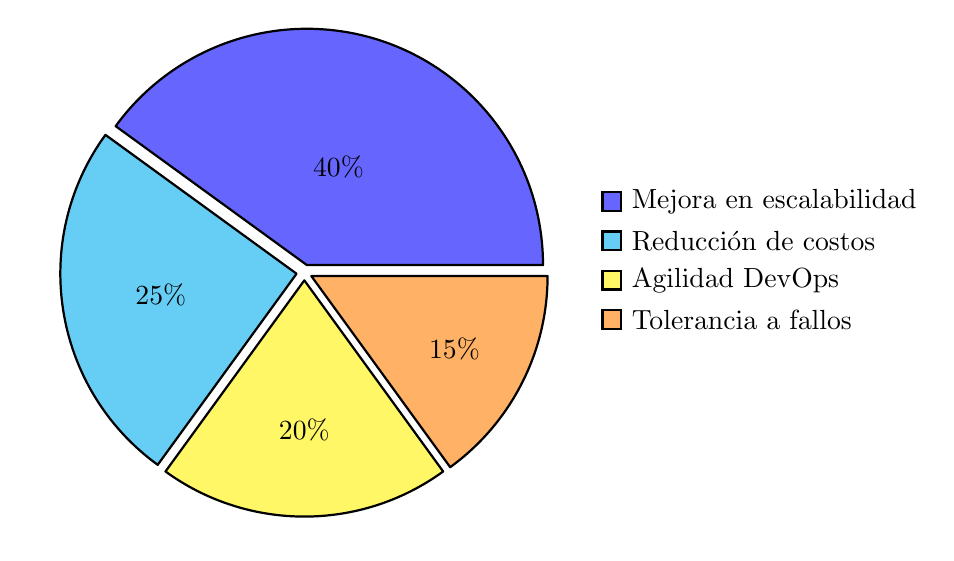
\begin{tikzpicture}
\pie[text=legend,explode=0.1]{40/Mejora en escalabilidad, 25/Reducción de costos, 20/Agilidad DevOps, 15/Tolerancia a fallos}
\end{tikzpicture}
\caption{Motivaciones de la Migración}
\label{fig:migration_motives}
\end{figure}

\section{Comparativa: Monolitos vs Microservicios}

\subsection{Caracterización Detallada}
La Tabla~\ref{tab:architecture_comparison} destaca diferencias clave entre ambas arquitecturas:

\begin{table}[htbp]
\caption{Comparativa Detallada de Arquitecturas}
\label{tab:architecture_comparison}
\begin{tabular}{|p{2.5cm}|p{2.5cm}|p{2.5cm}|}
\hline
\textbf{Característica} & \textbf{Monolítica} & \textbf{Microservicios} \\
\hline
Escalabilidad & Limitada & Altamente dinámica \\
Despliegue & Complejo & Independiente \\
Tolerancia a Fallos & Baja & Alta \\
Mantenimiento & Alta complejidad & Modular \\
Tecnologías & Homogéneas & Diversas \\
\hline
\end{tabular}
\end{table}

\begin{figure}[htbp]
\centering
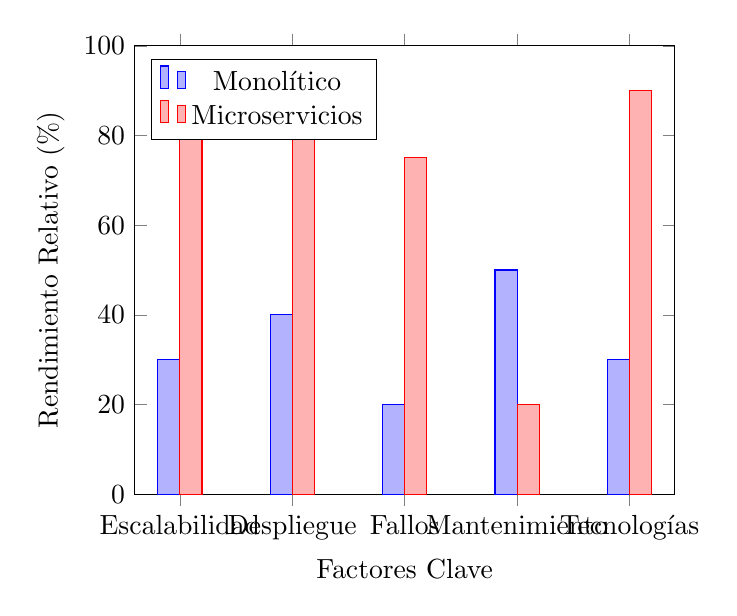
\begin{tikzpicture}
\begin{axis}[
    xlabel={Factores Clave},
    ylabel={Rendimiento Relativo (\%)},
    symbolic x coords={Escalabilidad, Despliegue, Fallos, Mantenimiento, Tecnologías},
    xtick=data,
    ybar=0pt,
    ymin=0,
    ymax=100,
    legend pos=north west,
    bar width=8pt
]
\addplot coordinates {(Escalabilidad,30) (Despliegue,40) (Fallos,20) (Mantenimiento,50) (Tecnologías,30)};
\addplot coordinates {(Escalabilidad,80) (Despliegue,90) (Fallos,75) (Mantenimiento,20) (Tecnologías,90)};
\legend{Monolítico,Microservicios}
\end{axis}
\end{tikzpicture}
\caption{Comparativa de Rendimiento}
\label{fig:comparison_chart}
\end{figure}

\section{Estrategias Avanzadas de Migración}

\subsection{Métodos Principales}
Las estrategias más eficaces incluyen:

\begin{itemize}
    \item \textbf{Strangler Pattern:} Reemplazo progresivo de componentes del monolito.
    \item \textbf{Migración Incremental:} Construcción gradual de servicios.
    \item \textbf{Parallel Running:} Mantener sistemas antiguos y nuevos en paralelo.
    \item \textbf{Refactorización Selectiva:} Identificar módulos clave y separarlos.
\end{itemize}

\begin{figure}[htbp]
\centering
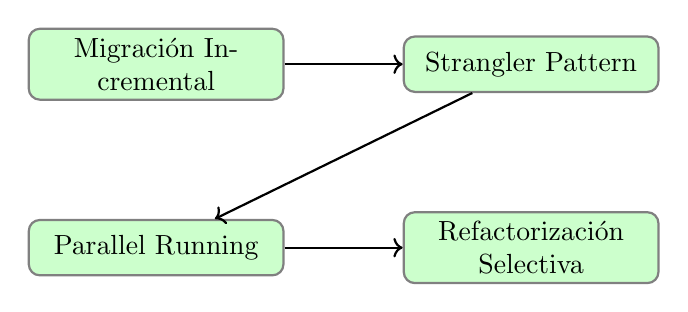
\begin{tikzpicture}[node distance=1.5cm]
\tikzset{
    strategy/.style={rectangle, draw=black!50, thick, fill=green!20, text width=3cm, text centered, rounded corners, minimum height=2em}
}
\node[strategy] (incremental) {Migración Incremental};
\node[strategy, right=of incremental] (strangler) {Strangler Pattern};
\node[strategy, below=of incremental] (parallel) {Parallel Running};
\node[strategy, right=of parallel] (refactoring) {Refactorización Selectiva};

\draw[thick,->] (incremental) -- (strangler);
\draw[thick,->] (strangler) -- (parallel);
\draw[thick,->] (parallel) -- (refactoring);
\end{tikzpicture}
\caption{Estrategias de Migración a Microservicios}
\label{fig:migration_strategies}
\end{figure}

\section{Herramientas para Migración}

\subsection{Plataformas de Contenerización}
\begin{itemize}
    \item Docker
    \item Kubernetes
    \item OpenShift
\end{itemize}

\subsection{Monitoreo y Observabilidad}
\begin{itemize}
    \item Prometheus
    \item Grafana
    \item Jaeger
\end{itemize}

\subsection{Orquestación y Gateway}
\begin{itemize}
    \item Kubernetes como orquestador.
    \item Istio y Linkerd como servicios mesh.
\end{itemize}

\begin{figure}[htbp]
\centering
\includegraphics[width=0.45\textwidth]{tools-diagram.jpg}
\caption{Ecosistema de Herramientas para Microservicios}
\label{fig:tools_ecosystem}
\end{figure}

\section{Casos de Estudio Avanzados}

\subsection{Netflix: Transformación Global}
Resultados clave:
\begin{itemize}
    \item Más de 1000 microservicios independientes.
    \item Disponibilidad del 99.99\%.
    \item Despliegues ágiles con frecuencia diaria.
\end{itemize}

\subsection{Spotify: Escalabilidad en Música Digital}
Beneficios observados:
\begin{itemize}
    \item Separación modular por características (playlists, recomendaciones, streaming).
    \item Reducción de tiempo de inactividad.
\end{itemize}

\section{Conclusiones y Proyección Futura}

\begin{enumerate}
    \item Migración a microservicios mejora agilidad y resiliencia.
    \item Retos incluyen complejidad en la gestión de servicios.
    \item Herramientas como Kubernetes e Istio son fundamentales.
\end{enumerate}

\begin{figure}[htbp]
\centering
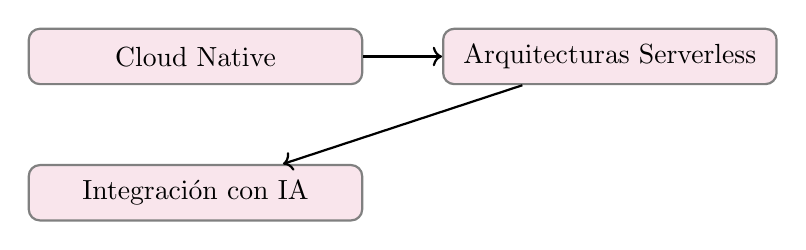
\begin{tikzpicture}
\tikzset{
    future/.style={rectangle, draw=black!50, thick, fill=purple!10, text width=4cm, text centered, rounded corners, minimum height=2em}
}
\node[future] (cloud) {Cloud Native};
\node[future, right=of cloud] (serverless) {Arquitecturas Serverless};
\node[future, below=of cloud] (ai) {Integración con IA};

\draw[thick,->] (cloud) -- (serverless);
\draw[thick,->] (serverless) -- (ai);
\end{tikzpicture}
\caption{Tendencias Futuras en Arquitecturas de Software}
\label{fig:future_trends}
\end{figure}

\bibliographystyle{IEEEtran}
\bibliography{referencias}

\end{document}
